\subsection{Deep Feedforward Models}
\label{sec:deep1}

Linear models directly map from inputs to predictions.
Assuming the inputs stay the same, the next step in neural network evolution
should be to add hidden layers.
The reasoning behind this is the increased capability of the model to learn intermediate
feature representations, which in turn should enable more accurate predictions.
This section examines application of deep feedforward networks to the problem
of engagement prediction.
Model architectures are introduced in Chapter~\ref{sub:deep1_architecture}, 
before the training process is detailled in Chapter~\ref{sub:deep1_training}.
Finally, results and accompanying analysis are presented in Chapter~\ref{sub:deep1_performance}.

\subsubsection{Model architecture}
\label{sub:deep1_architecture}

Model architecture for the deep feedforward networks is similar to linear models
in that model inputs and outputs are the same.
The main difference is the addition of hidden layers inbetween inputs and outputs.
Fully-connected feedforward layers (see ch.~\ref{sub:dl_concepts}) are chosen,
because they constitute the sole reasonably applicable layer architecture.
More complex layer architectures like recurrent or convolutional layers require
temporal or local relations between input features.
Examples for such relations would be images (local relations between pixels)
or time-series data (obvious temporal relation).
The main question that arises is how many hidden layers should be inserted.
Additionally, the number of neurons in hidden layers has to be determined.
No strict rules exist to answer this question, but heuristics have been developed
by long-time deep learning practicioners~\footnote{\url{http://www.heatonresearch.com/2017/06/01/hidden-layers.html}}.
In any case, experimentation is required to find a suitable architecture for a distinct problem setting.
Thus, several architectures were tested for model selection in this work.
Obvious evaluation criteria are model performance on training and validation data,
as well as total training time.

\begin{table}
\begin{tabular}{llrr}
\toprule
Hidden layers & Hidden units & Classification loss & Regression loss \\
\midrule
2 & 16 & 0.8203 & 2,593.2 \\
2 & 32 & 0.7502 & 2,520.2 \\
2 & 64 & 0.7346 & 2,509.9 \\
3 & 16 & 0.7888 & 2,529.9 \\
3 & 32 & 0.7430 & 2,557.3 \\
3 & 64 & 0.7160 & 2,465.1 \\
4 & 16 & 0.7792 & 2,588.5 \\
4 & 32 & 0.7261 & 2,477.5 \\
4 & 64 & \textbf{0.7088} & 2,435.8 \\
5 & 64 & 0.7128 & \textbf{2,386.1} \\
6 & 64 & 0.7016 & 2,410.1 \\
\bottomrule
\end{tabular}
\caption{Summary of model selection results}
\label{tab:dm1_selection_results}
\end{table}

Experimentation for classification and regression models was conducted on the
celebrity data set, because it contains the smallest number of training examples
and is thus most prone to overfitting.
In order to preserve comparability, the same settings were used for each architecture.
Models were trained for 50 (classification) respectively 100 (regression) epochs
on identical training examples.
Tested variants included two to six hidden layers with the same number of hidden
units in each layer, namely 16, 32 and 64 neurons.
Some architectures for very deep networks (five or six hidden layers) were omitted
when it became obvious that layers with 64 neurons showed the most promising
performance.
Table~\ref{tab:dm1_selection_results} summarizes results for the experiments.
As expected, increases in both number of hidden layers and units improve
performance.
However, adding units yields generally leads to higher performance increases than
simply adding layers.
Moreover, adding more hidden layers increases total training time more than
adding units.
Including more than four hidden layers only leads to minor performance improvement for
the classification setting.
Also, a more unstable training process was observed, sometimes resulting in quickly overfitting
to the training data.
Hence, the configuration consisting of four layers with 64 neurons each was
chosen for models in this thesis.
The regression setting proved to be a bit more robust regarding the number of
hidden layers, so that an additional layer could be inserted here.

\begin{figure}[h]
\begin{subfigure}{.4\textwidth}
  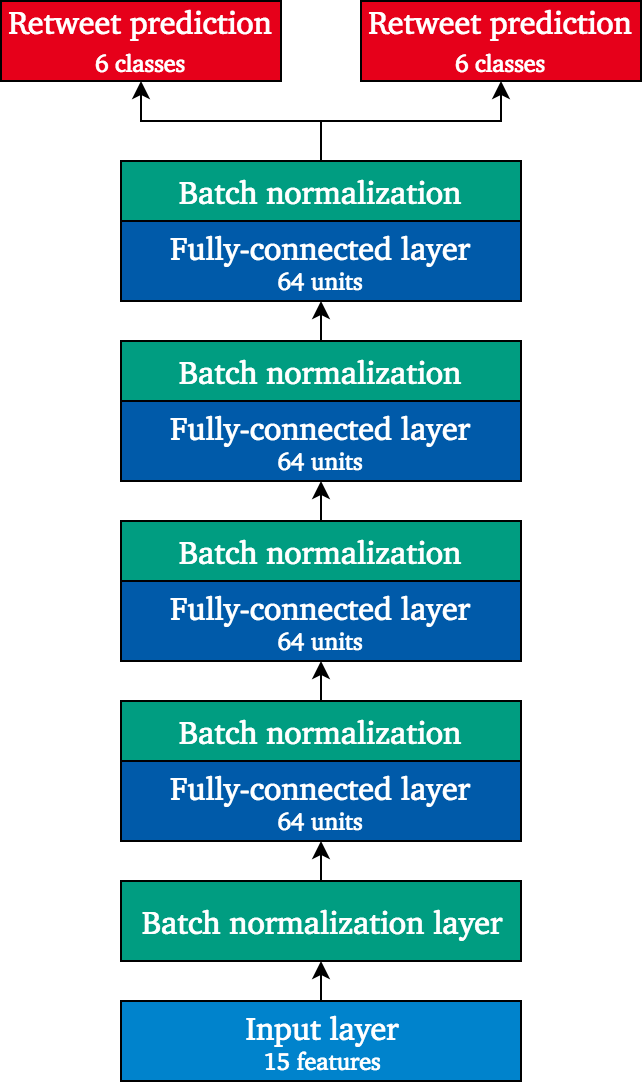
\includegraphics[width=.95\linewidth]{img/deep_1_class_architecture}
  \caption{Classification model}
  \label{fig:deep1_architecture_1}
\end{subfigure}%
\begin{subfigure}{.4\textwidth}
  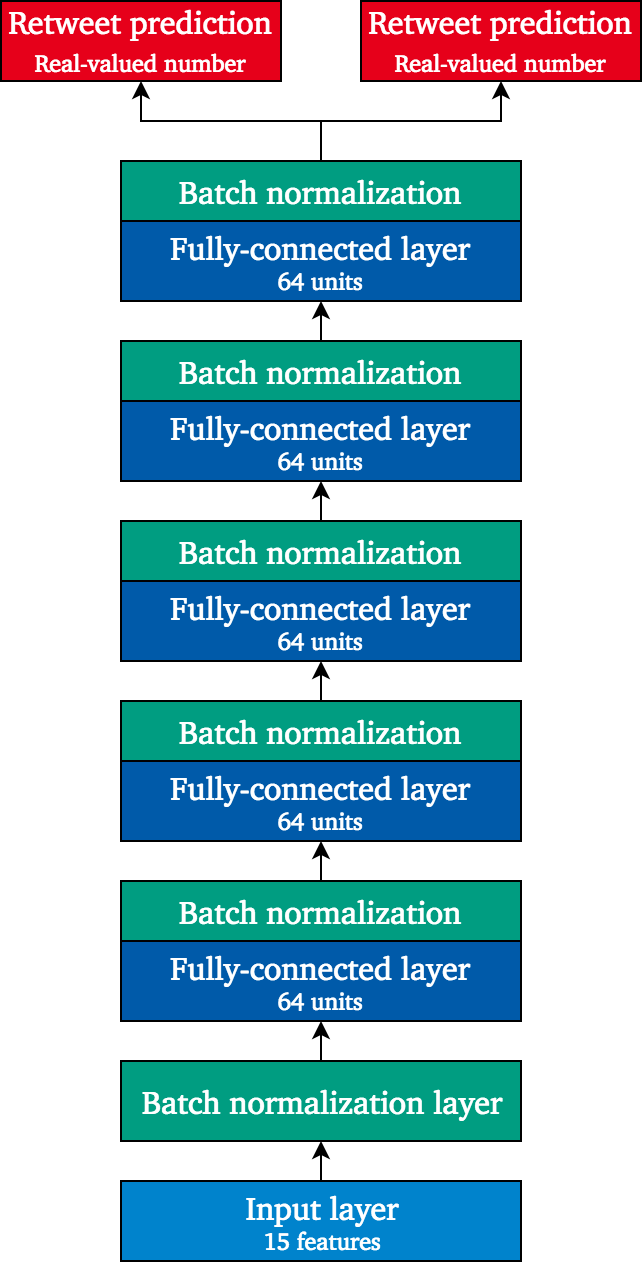
\includegraphics[width=.95\linewidth]{img/deep_1_regr_architecture}
  \caption{Regression model}
  \label{fig:deep1_architecture_2}
\end{subfigure}
\caption{Architecture of deep feedforward network}
\label{fig:deep1_architecture}
\end{figure}

Fig.~\ref{fig:deep1_architecture} shows the final neural network architectures
for this section.
Input features and output types (including classes) are identical to the ones
used in linear models (see ch.~\ref{sub:lin_architecture}).
As before, inputs are normalized using batch normalization, which is also applied
after each fully-connected layer.
Citing Chapter~\ref{sub:dl_developments}, batch normalization speeds up the
training process by decreasing the range of weight values without sacrificing
model performance.
Moreover, it helps to avoid overfitting, which is more prone to occur in models
containing many learnable parameters.
For the larger data sets, further regularization had to be added in order prevent overfitting.
More specifically, dropout was inserted after each fully-connected layer, where
the probability of keeping a neuron was set to 50\% (see ch.~\ref{sub:dl_developments}).

\subsubsection{Training process}
\label{sub:deep1_training}

As mentioned above, training setting remain mostly unchanged.
The same training and validation splits were used for all data sets, i.e.,
for the singular data sets 10\% of all examples were separated for validation.
The validation set for the combined data set comprised 10,000 examples.
Furthermore, optimization algorithm and cost functions were identical to the ones
used for training linear models.
To recap, adaptive moment estimation (Adam) was used for optimizing
categorical cross-entropy (classification models) and mean absolute error (regression
models) cost functions.
Because faster convergence was observed on the regression task, the total number
of iterations was decreased from 150 to 100 iterations.
Classification models were still trained for a total of 50 iterations each.

\subsubsection{Model performance}
\label{sub:deep1_performance}

This section will list results of training deep feedforward networks on the task
of engagement prediction.
First, general performance metrics will be presented, before subsequent paragraphs
analyze the results for both regression and classification approaches in more
detail.

\begin{table}
  \begin{tabular}{lrrrrrrr}
    \toprule
    & \multicolumn{4}{l}{Classification} & \multicolumn{3}{l}{Regression} \\
    \midrule
    Data set & CCE & Acc & Ret Acc & Fav Acc & MAE & Ret MAE & Fav MAE \\
    \midrule
    Celebrities & 0.71 & 70.29\% & 66.30\% & 74.28\% & 2,345.91 & 1,142.60 & 3,549.23 \\
    Politicians & 0.81 & 64.75\% & 63.37\% & 66.12\% & 414.68 & 230.60 & 598.76 \\
    Companies & 0.72 & 70.07\% & 72.38\% & 67.76\% & 20.57 & 11.54 & 29.61 \\
    Combined & 1.03 & 55.50\% & 57.75\% & 53.25\% & 549.93 & 210.71 & 889.16 \\
    \bottomrule
  \end{tabular}
  \caption{Summary of results for deep feedforward network}
  \label{tab:deep1_results}
\end{table}

Table~\ref{tab:deep1_results} summarizes performance metrics across all data
sets for classification and regression task.
The metrics were calculated using unseen data, i.e., the held-out validation
set.
On the smaller data sets, performance increases considerably, i.e.,
smaller values are found for both cost functions.
Regarding the classification task, accuracy improves between 10 and 20\%, such
that 65 to 70\% of validation examples are labeled correctly by the classifier.
Here, the deep feedforward network yields the largest improvement on celebrity
tweets, which interestingly are also classified most accurately among all data sets.
This is in contrast to linear model results, where performance was worst on this
data set.
Except for politician data, performance increases are slightly higher for favorite
classification.
However, relations between both classification tasks remain unchanged, i.e.,
retweets are more accurately classified for celebrities and politicians.
Concerning the regression task, MAE values are lowered by 12 (politicians) to
33\% (celebrities).
These improvements are mainly driven by strong decreases in favorite MAE values,
which are higher for all three data sets.
For the combined data set, results are only slightly better compared to using
linear models.
Interestingly, performance on the favorite regression task does not improve
at all.
This is surprising, since one would expect larger performance increases when
adding more data.
Overall, results of appying deep feedforward networks to structured inputs
yield more compelling results than using linear models.
Nevertheless, room for further improvements is definitely given.
In order to understand the observed results better, both classification and 
regression performance will be analyzed further in the following paragraphs.

\begin{figure}[h]
\begin{subfigure}{.5\textwidth}
  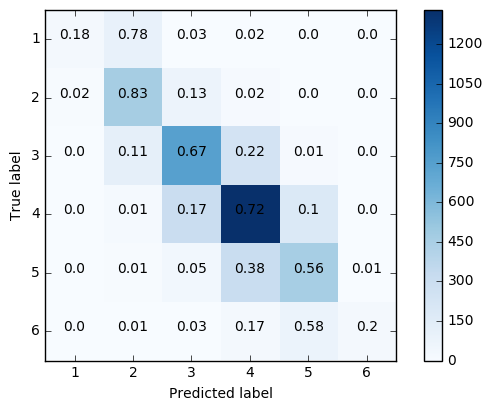
\includegraphics[width=.95\linewidth]{img/celeb_d1_cm_retweets}
  \caption{Celebrity data set}
  \label{fig:retw_distr_sub1}
\end{subfigure}%
\begin{subfigure}{.5\textwidth}
  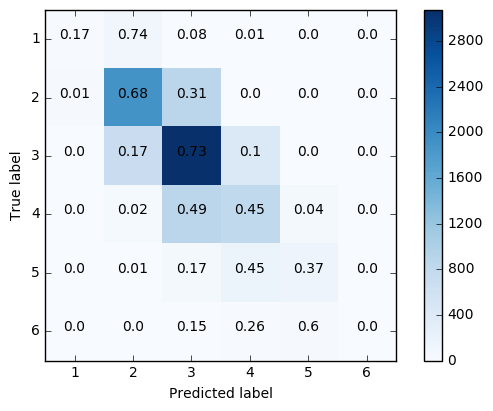
\includegraphics[width=.95\linewidth]{img/polit_d1_cm_retweets}
  \caption{Politician data set}
  \label{fig:retw_distr_sub2}
\end{subfigure}
\begin{subfigure}{.5\textwidth}
  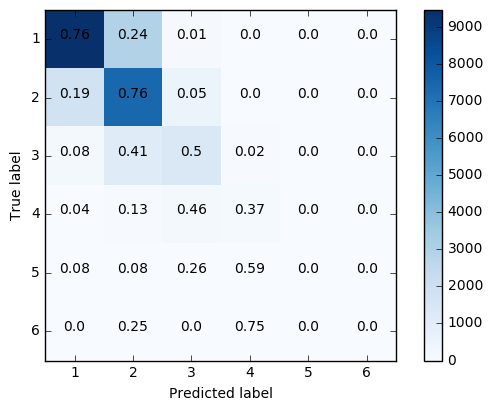
\includegraphics[width=.95\linewidth]{img/corp_d1_cm_retweets}
  \caption{Company data set}
  \label{fig:retw_distr_sub3}
\end{subfigure}%
\begin{subfigure}{.5\textwidth}
  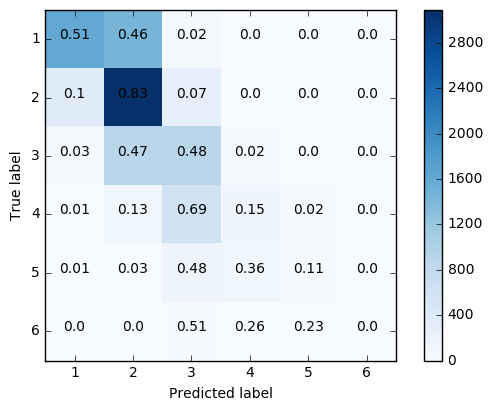
\includegraphics[width=.95\linewidth]{img/comb_d1_cm_retweets}
  \caption{Combined data set}
  \label{fig:retw_distr_sub4}
\end{subfigure}%
\caption{Confusion matrices for deep feedforward classification models}
\label{fig:d1_cm}
\end{figure}

Fig.~\ref{fig:d1_cm} shows confusion matrices for retweet classification on all
data sets.
Again, the matrices look similar for favorite prediction and are omitted
here for the sake of brevity.
In general, more validation examples are classified correctly for the three
smaller data sets, i.e., percentages on the main diagonals are higher.
For the celebrity data set it holds true that classes around the median of the
distribution (class 4) are predicted more accurately than border classes.
However, predictions for these less common classes are less biased towards
the biggest class.
Instead, misclassifications mostly happen on behalf of neighboring classes (2 and 5),
which makes the predictions in a sense ``better''.
Both observations can also be made on the politician data set.
In addition, it has to be noted that class 6 is never predicted for politicians
and companies.
Reasons for this could be the small number of training examples from this class
or a lack of representational capability in the model.
Retweet predictions on the company data are still biased towards the first
two classes, which also occur most commonly in this data set.
Performance for theses classes is good, whereas the other classes are predicted
with accuracies of 50\% or below.
These observed results are better compared to applying linear models, but still
not satisfying.
As mentioned above, classes 5 and 6 are never predicted and thus, accuracy is
equal to zero here.
Similar results can be found for the combined data set.
Classes 1 and 2 are predicted best, class 3 predictions are also significantly
better than for linear models.
On the negative side, performance on classes 4, 5 and 6 is decreasing, which
points to an inability of the model to learn this wide-ranging class
distribution.

\begin{table}
  \begin{tabular}{lrrrrrrr}
    \toprule
    & \multicolumn{7}{c}{Actual retweets} \\
    \midrule
    Data set & 0 & 1-10 & 10-100 & 100-1k & 1-10k & 10-100k & >100k \\
    \midrule
    Celebrities & 17.2 & 26.9 & 92.3 & 281.5 & 1,762.6 & 18,707.9 & 135,543.6 \\
    Politicians & 17.5 & 16.7 & 35.8 & 238.9 & 2,185.0 & 15,758.5 & - \\
    Companies & 1.1 & 2.3 & 16.9 & 179.3 & 2,345.5 & 15,446.9 & - \\
    Combined & 0.4 & 5.2 & 32.0 & 233.6 & 2,088.3 & 21,919.0 & 86,217.9 \\
    \bottomrule
    \toprule
    & \multicolumn{7}{c}{Actual favorites} \\
    \midrule
    Data set & 0 & 1-10 & 10-100 & 100-1k & 1-10k & 10-100k & >100k \\
    \midrule
    Celebrities & 101.7 & 107.3 & 216.4 & 494.4 & 1,928.2 & 13,965.3 & 125,209.9 \\
    Politicians & 38.0 & 38.6 & 50.5 & 239.6 & 2,232.23 & 16,978.7 & 98,543.7 \\
    Companies & 2.6 & 3.3 & 15.1 & 194.1 & 1,743.7 & 18,657.8 & - \\
    Combined & 0.4 & 4.4 & 32.1 & 355.8 & 3,279.5 & 26,871.1 & 169,920.5 \\
    \bottomrule
  \end{tabular}
  \caption[Detailed regression results for deep feedforward networks]{Mean absolute errors for specific ranges of actual engagement}
  \label{tab:d1_regression_eval}
\end{table}

Analyzing regression results in more detail is helpful, especially when considering
that the MAE loss value represents an average over all validation examples.
In order to evaluate model performance in more detail, MAE values should thus be
observed separately for different ranges of actual engagement.
This evaluation approach effectively puts observed error magnitudes in relation
to actual engagement counts and further helps to determine in which ranges 
the model performs better than in others.
Table~\ref{tab:d1_regression_eval} shows results of such an analysis, with
engagement distributions separated into seven distinct regions.
These regions basically represent logarithmic bins with base 10, similar to
the bins used in classification models.
Dashes denote that no example in the given range was present in a respective
validation set.
As expected, mean absolute errors increase with rising actual engagement.
Put simply: the smaller the actual retweet or favorite count, the smaller the
average prediction error.
As Table~\ref{tab:deep1_results} showed, retweet predictions are generally more
accurate than favorite predictions.
This more detailed examination suggests the generally higher levels of favorite
counts as a possible reason for this observation.
Favorite distributions are effectively shifted to the right compared with their
retweet counterparts, thus putting more outliers into the mean calculation.
A similar explanation can be given for higher regression loss values on
celebrity and combined data set.
These are the only data sets that contain examples with very large engagement
counts, which act as outliers and thus have large influence on the mean
calculation.
The same biases found in classification models can also be identified for the
regression task, i.e., errors are comparably smaller in bins containing many data points.
For example, performance for the first three bins is comparably good on the company data
set, where errors are rather small.
This performance advantage diminishes for larger bins, performance is equal or
worse compared to the other data sets here.

This section concludes the results of applying deep feedforward networks to
the problem of engagement prediction. 
So far, only structured data was used as model input, namely by extracting
numeric and boolean features from tweet objects.
The next section introduces ways of incorporating the actual tweet content as
an additional input to more complex neural networks.

